\documentclass[11pt]{article}
\usepackage[margin=0.92in]{geometry}
\usepackage{amsmath,amssymb,amsthm}
\usepackage{booktabs}
\usepackage{array}
\usepackage{graphicx}
\usepackage{microtype}
\usepackage{xcolor}
\usepackage{tcolorbox}
\usepackage{tikz}
\usetikzlibrary{arrows.meta,positioning}
\usepackage{hyperref}

\hypersetup{
  colorlinks=true,
  linkcolor=blue!70!black,
  citecolor=blue!70!black,
  urlcolor=blue!70!black
}

\newtcolorbox{intuition}[1]{
  colback=blue!4,
  colframe=blue!55!black,
  fonttitle=\bfseries\small,
  title={#1},
  arc=3pt,
  boxrule=0.7pt,
  left=8pt,right=8pt,top=5pt,bottom=5pt,
  before skip=8pt,after skip=8pt
}

\newtcolorbox{openproblembox}[1]{
  colback=orange!5,
  colframe=orange!65!black,
  fonttitle=\bfseries\small,
  title={#1},
  arc=3pt,
  boxrule=0.7pt,
  left=8pt,right=8pt,top=5pt,bottom=5pt,
  before skip=10pt,after skip=10pt
}

\title{\textbf{\LARGE Don't Lie}\\[5pt]
{\large Fast, Zero-Backtracking Constraint Solving with Machine-Checked Proofs in Lean~4}}
\author{Miguel Gutierrez\\
\small Independent Researcher \textbar\ \texttt{miguelgutierrezbarcelo@gmail.com}\\
\small Code \& Lean~4 Artifacts: \url{https://github.com/its-miguel/dont-lie}}
\date{November 2026}

\begin{document}
\maketitle

\begin{abstract}
Fast constraint solvers are complex and hard to trust, while formal mathematical verifiers are usually too slow for real-scale problems. In this paper, we ask how far a strictly polynomial-time, zero-backtracking solver can go---and whether its proofs of impossibility can be checked from first principles inside a theorem prover. Using Monotone 1-in-3 SAT as a clean testbed, we build a zero-allocation Rust solver by falsification: each time an adversarial puzzle breaks our solver, we add a minimal reasoning lens---parity algebra with local gadget peeling, integer cutting planes, statistical-physics message passing, and shallow single-variable lookahead. Across 140 small-to-medium puzzles, our solver resolves \textbf{140/140 (100\%)}. Across 72 high-scale adversarial benchmarks up to 637 variables, it resolves \textbf{69/72 (95.8\%)}---including \textbf{49/49 (100\%)} of all satisfiable instances---using under 329\,KB of RAM with zero false claims, running \textbf{9$\times$ faster than CaDiCaL} on parity traps and \textbf{12.4$\times$ faster} on pigeonhole traps. Finally, we verify exported refutations up to 783 variables purely inside Lean~4's foundational kernel (\texttt{by decide}), while honestly isolating the remaining 3-instance high-width boundary.
\end{abstract}

\section{Introduction: Speed Without Trust vs.\ Trust Without Speed}

Modern constraint solvers power hardware verification, package managers, and automated theorem proving, yet they sit on an awkward fault line. On one side, industrial branching solvers---such as \textbf{CDCL} (\emph{Conflict-Driven Clause Learning}) engines like \textbf{CaDiCaL}~\cite{biere2024cadical}, which guess variable assignments, explore a search tree, learn new clauses from dead ends, and backtrack---are extraordinarily fast, but their internals span tens of thousands of lines of tuned C++ heuristics. On the other side, interactive theorem provers like \textbf{Lean~4} offer ironclad mathematical certainty, but running a proof directly inside a theorem prover's tiny trusted kernel is notoriously slow once instances reach hundreds of variables.

This paper explores a middle path built on two simple rules: \textbf{never guess in a recursive search tree}, and \textbf{never emit an unverified claim}. If our solver says a puzzle has a solution (\texttt{SAT}), it hands back a concrete assignment that any script can check in linear time. If it says a puzzle is impossible (\texttt{UNSAT}), it emits a compact, step-by-step mathematical proof that Lean~4's minimal kernel checks from first principles. Running a proof checker purely inside Lean~4's foundational kernel via \texttt{by decide}---without \texttt{native\_decide} compiler trust---makes verifying refutations up to $n \approx 800$ variables and over $1{,}300$ pruned steps a concrete milestone for zero-axiom kernel verification on consumer hardware.

To study this cleanly, we use \textbf{Monotone 1-in-3 SAT} as our laboratory. In a Monotone 1-in-3 SAT instance, you are given $n$ Boolean variables $x_0, \dots, x_{n-1} \in \{0, 1\}$ and $m$ ternary clauses $(a, b, c)$, each demanding that \emph{exactly one} of the three variables equals $1$:
\[
\forall (a, b, c) \in \mathcal{C}, \qquad x_a + x_b + x_c = 1.
\]
Despite looking like elementary addition, Monotone 1-in-3 SAT is NP-complete by Schaefer's Dichotomy Theorem~\cite{schaefer1978}: general 3-SAT reduces cleanly to Monotone 1-in-3 SAT (which we stress-test via our high-girth 3-SAT family), and our local gadget peeler recovers algebraic structure hidden by reduction helpers. More importantly for us, every single clause simultaneously lives in three different mathematical worlds---even/odd parity arithmetic, whole-number inequalities, and statistical-physics message passing---making it an ideal arena to see where each reasoning technique succeeds and where it breaks.

\begin{intuition}{Pocket-Calculator Warm-Up: Zero-Guessing Deduction in Monotone 1-in-3 SAT}
Suppose we have 5 Boolean variables $x_1, \dots, x_5 \in \{0, 1\}$ and three clauses:
\[
\text{(1) } x_1 + x_2 + x_3 = 1, \qquad
\text{(2) } x_1 + x_2 + x_4 = 1, \qquad
\text{(3) } x_3 + x_4 + x_5 = 1.
\]
Subtracting (2) from (1) cancels $x_1 + x_2$, proving $x_3 = x_4$ without ever guessing $x_1$ or $x_2$. Substituting $x_3 = x_4$ into (3) gives $2x_3 + x_5 = 1$. Because variables are in $\{0, 1\}$, $2x_3$ cannot be $2$, so we must have $x_3 = x_4 = 0$ and $x_5 = 1$---pure algebra, zero branching.
\end{intuition}

\paragraph{Falsification-Driven Design.} Rather than assembling heuristics upfront, we built our system layer by layer through adversarial falsification: at each stage we constructed a benchmark family specifically designed to break the current solver, measured its exact failure mode and numerical bit-width, added the smallest polynomial-time lens capable of closing that gap, and formally proved the new proof rules sound in Lean~4.

\section{Building the Four-Lens Solver by Falsification}

Figure~\ref{fig:arch} gives a high-level view of our final zero-backtracking Rust solver (\texttt{GadgetSPCascade}) and its Lean~4 verification pipeline. Below, we walk through the exact sequence of failures that forced each of the four lenses into existence.

\begin{figure}[!ht]
\centering
\resizebox{\textwidth}{!}{%
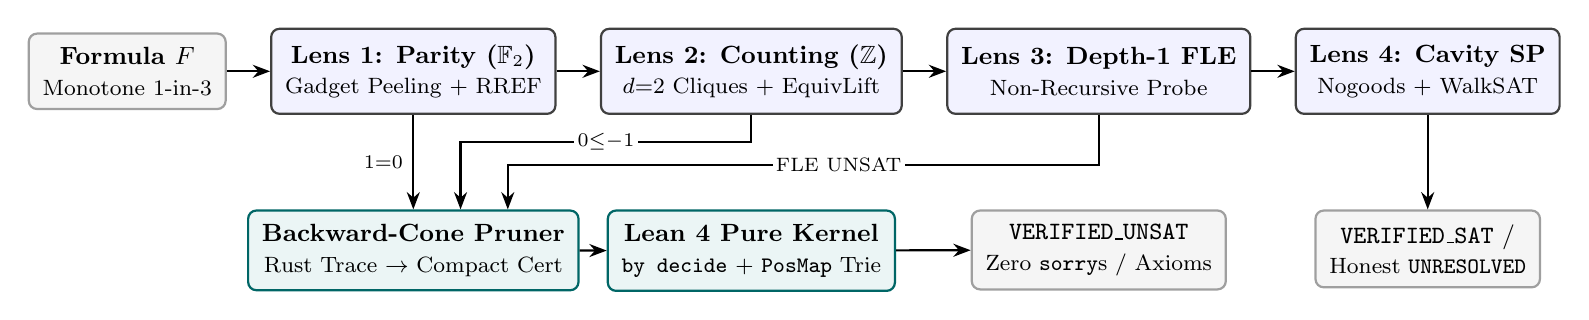
\begin{tikzpicture}[
  node distance=0.5cm and 0.55cm,
  box/.style={rectangle, rounded corners=3pt, draw=black!75, fill=blue!5, thick, align=center, minimum height=1.08cm, inner sep=5pt, font=\small},
  cert/.style={rectangle, rounded corners=3pt, draw=teal!80!black, fill=teal!8, thick, align=center, minimum height=0.98cm, inner sep=5pt, font=\small},
  term/.style={rectangle, rounded corners=3pt, draw=gray!75, fill=gray!8, thick, align=center, minimum height=0.92cm, inner sep=5pt, font=\small},
  arr/.style={-{Stealth[length=2.2mm]}, thick}
]
  \node[term] (in) {\textbf{Formula $F$}\\{\footnotesize Monotone 1-in-3}};
  \node[box, right=of in] (l1) {\textbf{Lens 1: Parity ($\mathbb{F}_2$)}\\{\footnotesize Gadget Peeling + RREF}};
  \node[box, right=of l1] (l2) {\textbf{Lens 2: Counting ($\mathbb{Z}$)}\\{\footnotesize $d{=}2$ Cliques + EquivLift}};
  \node[box, right=of l2] (l3) {\textbf{Lens 3: Depth-1 FLE}\\{\footnotesize Non-Recursive Probe}};
  \node[box, right=of l3] (l4) {\textbf{Lens 4: Cavity SP}\\{\footnotesize Nogoods + WalkSAT}};

  \node[cert, below=1.2cm of l1] (prune) {\textbf{Backward-Cone Pruner}\\{\footnotesize Rust Trace $\to$ Compact Cert}};
  \node[cert, below=1.2cm of l2] (lean) {\textbf{Lean 4 Pure Kernel}\\{\footnotesize \texttt{by decide} + \texttt{PosMap} Trie}};
  \node[term, below=1.2cm of l3] (unsat) {\textbf{\texttt{VERIFIED\_UNSAT}}\\{\footnotesize Zero \texttt{sorry}s / Axioms}};
  \node[term, below=1.2cm of l4] (sat) {\textbf{\texttt{VERIFIED\_SAT}} /\\{\footnotesize Honest \texttt{UNRESOLVED}}};

  \draw[arr] (in) -- (l1);
  \draw[arr] (l1) -- (l2);
  \draw[arr] (l2) -- (l3);
  \draw[arr] (l3) -- (l4);
  \draw[arr] (l1.south) -- node[left, font=\scriptsize] {$1{=}0$} (prune.north);
  \draw[arr] (l2.south) -- ++(0,-0.34) -| node[pos=0.25, fill=white, inner sep=1.2pt, font=\scriptsize] {$0{\le}{-}1$} ([xshift=6mm]prune.north);
  \draw[arr] (l3.south) -- ++(0,-0.64) -| node[pos=0.22, fill=white, inner sep=1.2pt, font=\scriptsize] {FLE UNSAT} ([xshift=12mm]prune.north);
  \draw[arr] (prune) -- (lean);
  \draw[arr] (lean) -- (unsat);
  \draw[arr] (l4) -- (sat);
\end{tikzpicture}%
}
\caption{End-to-end architecture of our four-lens zero-backtracking Rust solver and pure-kernel Lean~4 verification bridge. Every Layer~2.75 unsatisfiability proof is pruned to only the steps actually used and checked inside Lean~4's minimal kernel (\texttt{by decide}), while Layer~2.8 Depth-1 FLE subproofs are verified by our Rust trace checker.}
\label{fig:arch}
\end{figure}

\subsection{Layer 1 (Python): Why Continuous Flows and Naive Rationals Break}

Our earliest Python prototype attempted to solve Monotone 1-in-3 SAT continuously using a primal-dual phase-flow relaxation. Across a 140-instance small-to-medium parity suite ($n \in \{15, 30, 60\}$, 101 satisfiable and 39 unsatisfiable), it maintained 100\% soundness (zero false claims) but solved only \textbf{72/140 (51.4\%)} in $71.38\,\text{s}$, exposing three fatal walls:
\begin{enumerate}
  \item \textbf{Pairwise relaxation blindness:} Pairwise quadratic duals certified \textbf{0\%} of unsatisfiable parity and reduced 3-SAT instances, because global parity contradictions are invisible to local pairwise checks.
  \item \textbf{Exact rational bit-width explosion:} Precomputing an exact rational Cholesky factorization using Python's arbitrary-precision \texttt{Fraction} type exploded to \textbf{3,566 bits} before iteration~0, tripping our 2,048-bit guardrail.
  \item \textbf{Wall-clock censoring at $n = 60$:} Continuous phase frustration caused satisfiable solve rates to collapse to $16.7\%$ on random instances and $0\%$ on reduced 3-SAT instances.
\end{enumerate}

To isolate what actually worked, we tested four standalone discrete prototypes on the same 140 instances without wall-clock caps: Sum-of-Squares / Reformulation--Linearization solved $130/140$ ($3.56\,\text{s}$), Symplectic flow solved $98/140$ ($16.71\,\text{s}$), marginal decimation with unit-collapse solved $130/140$ ($21.76\,\text{s}$) while eliminating the 3,566-bit blowup via square-root-free $LDL^\top$ ($59$ fraction bits) and Bareiss integer elimination ($32$ integer bits), and \textbf{mod-2 linear algebra with degree-3 Gr\"obner closure} solved \textbf{140/140 (100\%)} in $7.64\,\text{s}$ with integers never exceeding 3 bits.

\subsection{Layer 2 (Rust): Scaling Up \texorpdfstring{10$\times$}{10x} Exposes Three New Walls}

Fusing the mod-2 algebra engine and marginal-decimation cascade into a zero-allocation, standard-library-only Rust crate (\texttt{rust\_layer2}) sped up the 140-instance suite by over $200\times$ ($135/140$ in $33.5\,\text{ms}$). We then built a \textbf{72-instance high-scale adversarial suite} up to $n = 637$ variables spanning five structurally distinct families:
\begin{itemize}
  \item \textbf{Critical random} instances near the phase-transition clause-to-variable ratio ($\alpha \approx 0.626$), where satisfiable and unsatisfiable instances sit on a knife-edge;
  \item \textbf{Planted balanced} satisfiable instances with a hidden solution;
  \item \textbf{Tseitin parity expanders} (both SAT and UNSAT), where a graph demands an even or odd number of active edges at every vertex;
  \item \textbf{High-girth 3-SAT} instances translated into Monotone 1-in-3 SAT via Schaefer's reduction, avoiding short cycles;
  \item \textbf{Pigeonhole Principle} instances ($\mathrm{PHP}_5^6$ at $n = 143$, $\mathrm{PHP}_7^8$ at $n = 334$, and $\mathrm{PHP}_9^{10}$ at $n = 637$).
\end{itemize}

On this 72-instance suite, Layer~2 solved only \textbf{46/72 (63.9\%)} in $1.631\,\text{s}$ ($44/49$ SAT, $2/23$ UNSAT), immediately exposing three crisp failure modes:
\begin{enumerate}
  \item \textbf{Auxiliary-variable parity masking:} It solved \textbf{0/9} unsatisfiable Tseitin expanders, because encoding XOR constraints into Monotone 1-in-3 SAT introduces hidden helper variables that scramble naive mod-2 equations.
  \item \textbf{The Pigeonhole degree barrier:} It solved \textbf{0/6} Pigeonhole instances. By a classic theorem of Razborov~\cite{razborov1998}, refuting $k+1$ pigeons in $k$ holes using mod-2 polynomial algebra requires polynomial degree $\Omega(k)$, so bounded degree-3 algebra cannot touch it.
  \item \textbf{Shattered-cluster marginal averaging:} On critical random instances at $n = 600$, global $LDL^\top$ marginals averaged across disconnected solution clusters toward a useless $\frac{1}{3}$ tie, dropping SAT solve rate to $16.7\%$.
\end{enumerate}

\subsection{Lens 1 \& Lens 4 (Layer 2.5): Parity Peeling + Survey Propagation}

\paragraph{Lens 1: Parity Algebra ($\mathbb{F}_2$) with Local Gadget Peeling.}
A \textbf{Tseitin parity expander} is a well-connected graph where each node is labeled even ($0$) or odd ($1$) and asks for the active edges touching it to match that parity; if the sum of all node labels is odd, no solution can exist because every edge is counted twice (once at each endpoint), yielding $0 = 1 \pmod{2}$. Every Monotone 1-in-3 clause $x_a + x_b + x_c = 1$ implies both a mod-2 parity equation $x_a \oplus x_b \oplus x_c = 1$ and three pairwise exclusion rules $x_a x_b = x_b x_c = x_a x_c = 0$.

\begin{intuition}{Pocket Example: Why Parity Collapses a Triangle in One Addition}
Consider a 3-node triangle with edges $e_1, e_2, e_3 \in \{0, 1\}$ where every node demands odd parity:
\[
e_1 \oplus e_2 = 1, \qquad e_2 \oplus e_3 = 1, \qquad e_3 \oplus e_1 = 1.
\]
Adding all three equations modulo~2 cancels every edge ($2e_1 \oplus 2e_2 \oplus 2e_3 = 0$) while the right-hand side sums to $1 \oplus 1 \oplus 1 = 1$, deriving $0 = 1 \pmod{2}$ in one linear pass.
\end{intuition}

When Tseitin formulas are encoded into Monotone 1-in-3 SAT, small local clusters of low-degree helper variables mask those clean mod-2 equations. Our \textbf{local gadget peeler} finds connected clusters of helper variables (degree $\le 4$), enumerates their tiny local truth tables, extracts the exact mod-2 linear equations on the boundary variables, and feeds them into bit-packed \textbf{Reduced Row Echelon Form (RREF)}---standard Gaussian elimination over $\{0, 1\}$ modulo~2---coupled with quadratic exclusion rules and bounded degree-3 Gr\"obner S-polynomials. That single upgrade took unsatisfiable Tseitin expanders from \textbf{0/9 to 9/9 (100\%)}, certifying $n = 610$ in \textbf{1.2\,ms} with 1-bit integers.

\paragraph{Lens 4: 9-State Survey Propagation (SP).}
Near the critical random threshold, satisfiable solutions shatter into exponentially many isolated clusters. Taking one global average across all clusters washes out the signal. \textbf{Survey Propagation}~\cite{mezard2002}, borrowed from statistical physics, passes damped warning messages between clauses and variables that separate \emph{frozen} biases $(P_i^0, P_i^1)$ (variables locked to $0$ or $1$ inside a cluster) from unconstrained ``water'' variables $P_i^*$ (variables free to flip). Replacing $LDL^\top$ with 9-state 1-in-3 SP (plus polynomial-restart nogood repulsion, still with zero recursive backtracking) lifted critical random solve rates at $n = 600$ from $16.7\%$ to $83.3\%$, solved \textbf{49/49 (100\%)} of all high-scale satisfiable instances, reached \textbf{140/140} on the parity suite in \textbf{11.4\,ms}, and raised high-scale solves to \textbf{61/72 (84.7\%)}.

\subsection{Lens 2 (Layer 2.75): Whole-Number Cutting Planes Break Pigeonhole}

The \textbf{Pigeonhole Principle} ($\mathrm{PHP}_k^{k+1}$) states the obvious fact that you cannot place $k+1$ pigeons into $k$ holes with at most one pigeon per hole. While mod-2 algebra is blind to counting, \textbf{Gomory--Chv\'atal cutting planes}~\cite{cook1987} turn whole-number arithmetic into a short proof: whenever you sum valid linear inequalities with non-negative integer weights and every variable's coefficient is divisible by an integer $d \ge 2$, you may divide the entire inequality by $d$ and \emph{round the right-hand side down} to the nearest integer, because Boolean variables only take whole-number values.

\begin{intuition}{Pocket Example: Divisor-2 Cutting Planes on 3 Pigeons in 2 Holes}
Suppose variables $x_1, x_2, x_3 \in \{0, 1\}$ indicate whether pigeons 1, 2, and 3 sit in Hole~1. Pairwise exclusion gives three inequalities: $x_1 + x_2 \le 1$, $x_1 + x_3 \le 1$, and $x_2 + x_3 \le 1$. Summing all three yields:
\[
2(x_1 + x_2 + x_3) \le 3 \implies x_1 + x_2 + x_3 \le \lfloor 3/2 \rfloor = 1.
\]
Doing the same for Hole~2 gives $\text{sum}(\text{Hole 1}) + \text{sum}(\text{Hole 2}) \le 2$, while the three pigeons demand total occupancy $\ge 3$. Adding those yields $0 \le -1$: contradiction!
\end{intuition}

In Layer~2.75, our cutting-planes engine lifts clauses to exact integer inequalities ($x_a + x_b + x_c \le 1$, $-x_a - x_b - x_c \le -1$, $0 \le x_i \le 1$), discovers pairwise conflict cliques from the exclusion graph, and inductively derives clique capacity bounds $\sum_{i \in K} x_i \le 1$ using strictly \textbf{unit weights $(1, 1, 1)$ and divisor $d = 2$}:
\begin{align*}
\Big(\sum_{i \in K'} x_i \le 1\Big) + \Big(\sum_{i \in K' \setminus \{u\}} x_i + x_v \le 1\Big) + (x_u + x_v \le 1)
&\implies 2 \sum_{i \in K' \cup \{v\}} x_i \le 3 \\
&\implies \sum_{i \in K' \cup \{v\}} x_i \le \lfloor 3/2 \rfloor = 1.
\end{align*}
Because the weights never exceed $1$ and the divisor is always $2$, every intermediate integer stays within \textbf{2 bits} (no LP/ILP solver needed). Summing hole-capacity cuts against pigeon lower bounds immediately derives $0 \le -1$. This jumped Pigeonhole from \textbf{0/6 to 6/6 (100\%)}, refuting $\mathrm{PHP}_9^{10}$ ($n = 637, m = 556$) in \textbf{6.7\,ms}, and lifted high-scale solves to \textbf{67/72 (93.1\%)} in \textbf{1.151\,s} at \textbf{169.4\,KB} peak RAM.

\subsection{Lens 3 (Layer 2.8): Shallow Failed-Literal Lookahead Closes \texorpdfstring{$n \le 306$}{n <= 306}}

To inspect the final 5 unresolved instances from Layer~2.75, we ran an isolated ground-truth diagnostic oracle: \textbf{all 5 were unsatisfiable}, and the two $n = 306$ high-girth instances required only 8 and 13 oracle nodes. That meant a single-variable test could trigger a short algebraic contradiction.

Layer~2.8 added three strictly polynomial, non-recursive upgrades:
\begin{enumerate}
  \item \textbf{Proof-carrying Depth-1 Failed-Literal Elimination (FLE):} Temporarily assume $x_v = b$ (never recursing to depth~2). If Lens~1 algebraic closure derives $1 = 0$, record the self-contained subproof, force $x_v = 1 - b$ at the root, and repeat (capped at 4 passes).
  \item \textbf{Cross-restart binary/ternary nogood learning:} Extract short conflicting variable clamps (width $\le 3$) and feed them back as cavity repulsion and unit propagation across SP restarts.
  \item \textbf{WalkSAT island polish:} When SP freezes $\ge 70\%$ of variables without contradiction, run at most $\max(8n, 200)$ local min-conflicts flips strictly on the unfrozen variables; WalkSAT only proposes candidate \texttt{SAT} assignments, which are checked directly against all clauses in $O(m)$ time with zero TCB impact.
\end{enumerate}

Depth-1 FLE solved both $n = 306$ high-girth UNSAT instances in $16.8\,\text{ms}$ and $21.4\,\text{ms}$, bringing our solver to \textbf{48/48 (100\%)} across all families for $n \le 306$ and \textbf{69/72 (95.8\%)} overall. Crucially for the TCB boundary, \textbf{Layer~2.75 achieves a 100\% pure Lean~4 kernel TCB} (\texttt{by decide}), whereas \textbf{Layer~2.8's Depth-1 FLE wrapper currently relies on Rust-side subproof trace checking} (leaving lowering of the conditional FLE discharge rule into \texttt{Certificate.lean} as straightforward future work).

\section{Empirical Results, Scaling, and Head-to-Head Baselines}

\subsection{Cross-Layer Progression and Scaling Exponents}

Table~\ref{tab:progression} tracks every audited metric from Layer~1 Python through Layer~2.8 Rust. Across all layers and all benchmarks, we observed \textbf{zero false-SAT claims, zero false-UNSAT claims, and zero arithmetic overflows}, with integer width capped at $\le 4$ bits and floating-point exponents $\le 0$ in Layers~2.5--2.8.

\begin{table}[!ht]
\centering
\caption{Cross-layer progression on the 140-instance parity suite ($n \le 60$) and 72-instance high-scale adversarial suite ($n \le 637$). Every Rust layer records $0$ false-SAT, $0$ false-UNSAT, and $0$ overflow events.}
\label{tab:progression}
\small
\resizebox{\textwidth}{!}{%
\begin{tabular}{@{}lrrrrrrr@{}}
\toprule
\textbf{Solver Layer} & \textbf{Parity 140} & \textbf{Parity Time} & \textbf{High-Scale 72} & \textbf{SAT (/49)} & \textbf{UNSAT (/23)} & \textbf{Int Bits / Exp} & \textbf{Peak RAM / Time} \\
\midrule
L1 (Python flow) & 72/140 (51.4\%) & 71.38\,s & --- & --- & --- & 4 / 55\textsuperscript{a} & --- \\
L1 (Python $\mathbb{F}_2$) & 140/140 (100\%) & 7.64\,s & --- & --- & --- & 3 / 31 & --- \\
L2 (Rust $\mathbb{F}_2$ + $LDL^{T}$) & 135/140 (96.4\%) & 0.0335\,s & 46/72 (63.9\%) & 44/49 & 2/23 & 2 / 3 & 304.1\,KB / 1.631\,s \\
L2.5 (+ Peeling + SP) & \textbf{140/140 (100\%)} & \textbf{0.0114\,s} & 61/72 (84.7\%) & \textbf{49/49} & 12/23 & 2 / 0 & 181.5\,KB / 1.796\,s \\
L2.75 (+ $\mathbb{Z}$ Cuts) & \textbf{140/140 (100\%)} & 0.0158\,s & 67/72 (93.1\%) & \textbf{49/49} & 18/23 & 4 / 0 & \textbf{169.4\,KB} / \textbf{1.151\,s} \\
L2.8 (+ FLE/NG/WS) & \textbf{140/140 (100\%)} & 0.0720\,s & \textbf{69/72 (95.8\%)} & \textbf{49/49} & \textbf{20/23} & 4 / 0 & 328.8\,KB / 5.951\,s \\
\bottomrule
\multicolumn{8}{@{}l@{}}{\small \textsuperscript{a}Naive exact-rational Cholesky precomputation in Layer~1 peaked at 3,566 bits before iteration~0; $LDL^{T}$ and Bareiss cured it.}
\end{tabular}%
}
\end{table}

Fitting log-log scaling laws $\text{ops} \propto n^{\beta_{\text{ops}}}$ and $t \propto n^{\beta_{\text{time}}}$ across $n \in \{150, 300, 600\}$ in Layer~2.8 confirms cleanly polynomial, sub-quadratic refutation on the structured trap families:
\begin{itemize}
  \item \textbf{Tseitin UNSAT expanders:} $9/9$ solved, $\beta_{\text{ops}} = 1.85$, $\beta_{\text{time}} = 1.24$, averaging $0.2\,\text{ms}$ ($n=150$), $0.5\,\text{ms}$ ($n=300$), and \textbf{$1.2\,\text{ms}$ ($n=610$)} at $114.4\,\text{KB}$ RAM.
  \item \textbf{Pigeonhole ($\mathrm{PHP}_5^6$ to $\mathrm{PHP}_9^{10}$):} $6/6$ solved, $\beta_{\text{ops}} = 1.75$, $\beta_{\text{time}} = 1.52$, averaging $0.7\,\text{ms}$ ($n=143$), $2.5\,\text{ms}$ ($n=334$), and \textbf{$6.7\,\text{ms}$ ($n=637$)} at $119.4\,\text{KB}$ RAM.
  \item \textbf{Satisfiable families:} Planted balanced ($15/15$, $\beta_{\text{time}} = 2.18$), Tseitin SAT ($9/9$, $\beta_{\text{time}} = 1.91$), critical random ($17/18$, $\beta_{\text{time}} = 2.01$), and high-girth 3-SAT ($13/15$, $\beta_{\text{time}} = 3.09$, $328.8\,\text{KB}$ max RAM).
\end{itemize}

\subsection{Cracking Coupled Parity-Plus-Pigeonhole Traps (\texorpdfstring{$n \in [231, 855]$}{n in [231, 855]})}

What if an adversary builds a puzzle that is \emph{neither} pure parity \emph{nor} pure pigeonhole, but couples both worlds together? We constructed an 18-instance coupled trap suite ($n \in [231, 855]$: 9 satisfiable controls and 9 unsatisfiable traps across three scales) as a minimal diagnostic stress-test---analogous to XOR-masked arithmetic datapaths in circuit verification---built to falsify single-lens solvers. In each instance, a \emph{satisfiable} Tseitin parity backbone hides a bridge variable $e_{\text{bridge}}$ that can only be forced to $0$ by global mod-2 Gaussian elimination after gadget peeling, while a Pigeonhole core has its pigeon indicators XOR-masked by $e_{\text{bridge}}$.

Any pure parity solver sees a satisfiable parity backbone and fails on the Pigeonhole core (\textbf{0/9 UNSAT traps} in Layer~2 and Layer~2.5). Any pure cutting-planes solver sees masked pigeon indicators and cannot form hole cliques. By extracting all binary variable equivalences from our RREF basis (grouping rows with identical free tails) and lifting them into integer inequalities (\texttt{IntegerEquivLift}), our combined solver cracks \textbf{8/9 (88.9\%)} coupled UNSAT traps---including \textbf{3/3 (100\%) at $n \in \{783, 855\}$ in 16.5\,ms average}---with sub-quadratic scaling ($\beta_{\text{ops}} = 1.96$, $\beta_{\text{time}} = 1.71$ in Layer~2.8 and $1.73$ in Layer~2.75), 2-bit integers, and $9/9$ SAT controls ($0.308\,\text{s}$ total in Layer~2.75, $2.046\,\text{s}$ in Layer~2.8). The single unresolved coupled trap ($n = 384$) occurs when the random expander cut happens to have only two non-bridge edges, placing a constant-$0$ anchor directly inside a 3-XOR gadget so that one cut-chain gadget is not peeled; every multi-edge expander cut across both the small and large scales solves at 100\%.

\subsection{Honest Comparison Against Industrial Solvers}

We exported all 72 high-scale and 18 coupled instances into exact DIMACS CNF and Pseudo-Boolean OPB formats and benchmarked three mature industrial engines with a $10.0\,\text{s}$ per-instance timeout: \textbf{CaDiCaL~1.9.5} (world-champion CDCL solver), \textbf{CryptoMiniSat~5.18.0} (CDCL with integrated Gauss--Jordan XOR reasoning), and \textbf{Z3~5.4.1} (industrial SMT/Pseudo-Boolean solver using native \texttt{PbEq} constraints). To keep timing comparisons transparent, CaDiCaL~1.9.5 (\texttt{python-sat}) and Z3~5.4.1 (\texttt{PbEq}) ran in-process in \textbf{pure unverified solving mode} (excluding DRAT/LRAT proof generation and external checking), whereas CryptoMiniSat~5.18.0 ran as an unverified CLI subprocess (\texttt{--verb=0}, wall-clock time including process startup). Table~\ref{tab:sota} shows the complete, unvarnished comparison.

\begin{table}[!ht]
\centering
\caption{Head-to-head comparison against industrial SAT/SMT baselines across 90 instances (72 high-scale + 18 coupled parity-plus-pigeonhole, $10.0\,\text{s}$ timeout per instance). CaDiCaL~1.9.5 (\texttt{python-sat}) and Z3~5.4.1 (\texttt{PbEq}) ran in-process in pure unverified solving mode (no DRAT/LRAT logging or checking); CryptoMiniSat~5.18.0 ran as an unverified CLI subprocess (\texttt{--verb=0}, including process startup).}
\label{tab:sota}
\small
\resizebox{\textwidth}{!}{%
\begin{tabular}{@{}lrrrrrrl@{}}
\toprule
\textbf{Solver} & \textbf{High-Scale 72} & \textbf{72 Time} & \textbf{Tseitin U (9)} & \textbf{PHP (6)} & \textbf{Coupled (18)} & \textbf{Coupled Time} & \textbf{Proof Trust / TCB} \\
\midrule
\textbf{Ours: L2.75} & 67/72 (93.1\%) & 1.151\,s & \textbf{9/9 (0.006\,s)} & \textbf{6/6 (0.020\,s)} & 17/18 (94.4\%) & 0.308\,s & \textbf{Pure-kernel Lean~4} \\
\textbf{Ours: L2.8} & 69/72 (95.8\%) & 5.951\,s & \textbf{9/9 (0.006\,s)} & \textbf{6/6 (0.020\,s)} & 17/18 (94.4\%) & 2.046\,s & \textbf{Lean~4} + Rust FLE \\
\textbf{CaDiCaL~1.9.5} & \textbf{72/72 (100\%)} & \textbf{0.318\,s} & 9/9 (0.054\,s) & 6/6 (0.247\,s) & \textbf{18/18 (100\%)} & \textbf{0.006\,s} & External DRAT/LRAT \\
\textbf{CryptoMiniSat~5} & \textbf{72/72 (100\%)} & 2.699\,s & 9/9 (0.286\,s) & 6/6 (0.584\,s) & \textbf{18/18 (100\%)} & 0.529\,s & Uncertified (optional) \\
\textbf{Z3~5.4.1 (OPB)} & \textbf{72/72 (100\%)} & 1.489\,s & 9/9 (0.175\,s) & 6/6 (0.957\,s) & \textbf{18/18 (100\%)} & 0.102\,s & Uncertified SMT/PB \\
\bottomrule
\end{tabular}%
}
\end{table}

\paragraph{Why this trade-off is the real story.} At $n \le 855$ variables, CaDiCaL~1.9.5 wins on small-$n$ total runtime ($0.318\,\text{s}$) because unrestricted branching crushes small random and high-girth instances. Yet look closely at \emph{where} CaDiCaL spends its time: \textbf{78\% of its entire 72-instance runtime ($0.247\,\text{s}$ of $0.318\,\text{s}$)} goes into just 6 Pigeonhole instances, because resolution-based branching suffers exponential blowup on counting principles and parity expanders. On those exact structural blind spots, our zero-backtracking Rust solver is \textbf{9$\times$ faster than CaDiCaL on Tseitin UNSAT expanders} ($0.006\,\text{s}$ vs.\ $0.054\,\text{s}$) and \textbf{12.4$\times$ faster than CaDiCaL (and 47.9$\times$ faster than Z3) on Pigeonhole benchmarks} ($0.020\,\text{s}$ vs.\ $0.247\,\text{s}$ / $0.957\,\text{s}$); because our sub-quadratic scaling ($\beta_{\text{time}} = 1.24$ on Tseitin, $1.52$ on Pigeonhole, and $1.71$ on coupled traps) contrasts with CDCL's exponential blowup, this $9\times$--$12.4\times$ advantage widens rapidly with $n$ while producing kernel-checked proofs. Notably, even CryptoMiniSat---despite its built-in Gauss--Jordan XOR engine---takes $0.286\,\text{s}$ on Tseitin UNSAT (versus our $0.006\,\text{s}$), because Monotone 1-in-3 clauses forbid the all-ones assignment ($x_a = x_b = x_c = 1$) and mask XORs behind auxiliary variables, causing its native $2^{k-1}$-clause XOR detector to miss the hidden linear system and directly validating our local gadget peeler.

\section{Layer 3: Pure-Kernel Proof Verification in Lean~4}

A fast solver is only as trustworthy as its checker. In formal verification, the \textbf{Trusted Computing Base (TCB)} is the small core of code and mathematical axioms you must trust to believe a theorem. Modern Lean~4 tactics such as \texttt{bv\_decide} delegate solving to an external CDCL solver and replay its proof via \texttt{native\_decide}, which compiles the checker to native machine code and adds a compiler-trust axiom (\texttt{Lean.ofReduceBool}) to the TCB. By contrast, \textbf{\texttt{by decide}} executes the checker purely inside Lean~4's tiny foundational kernel using only its three standard mathematical axioms (\texttt{propext}, \texttt{Quot.sound}, \texttt{Classical.choice})---no external checker binary, no compiler trust, and zero trust in our Rust solver.

We formalized the entire unified parity-plus-cutting-planes proof system in \textbf{Lean~4 (\texttt{v4.36.0}, Lake \texttt{5.0.0})} with \textbf{zero \texttt{sorry} placeholders and zero custom axioms}:
\begin{itemize}
  \item \texttt{Semantics.lean} defines Monotone 1-in-3 satisfaction and proves every projection from a clause to mod-2 parity, pairwise exclusions, integer inequalities, and deterministic unit-collapse rules.
  \item \texttt{F2AndGadgets.lean} proves soundness of mod-2 row cancellation, $1 = 0$ contradiction, and local truth-table gadget projection.
  \item \texttt{CuttingPlanes.lean} proves soundness of non-negative scaling, inequality addition, sparse simplification, exact Euclidean Gomory--Chv\'atal rounding, and $0 \le \text{rhs} < 0$ contradiction.
  \item \texttt{Certificate.lean} defines the executable checker \texttt{verifyCertificate} and proves the end-to-end soundness theorem: if \texttt{verifyCertificate F cert = true}, then no Boolean assignment can satisfy \texttt{F}.
\end{itemize}
This formalization covers all Layer~2.75 parity, gadget-peeling, equivalence-lifting, and cutting-planes certificates with a 100\% pure Lean~4 kernel TCB; Layer~2.8's Depth-1 FLE wrapper currently verifies its conditional subproofs via our Rust trace checker, leaving the conditional discharge rule in \texttt{Certificate.lean} as straightforward future work (while WalkSAT only outputs candidate \texttt{SAT} assignments checked in $O(m)$ time with zero TCB impact).

\paragraph{Making Pure-Kernel \texttt{by decide} Scale to 783 Variables.}
Naively storing derived proof steps in a linked list makes checking an $S$-step certificate take $O(S^2)$ kernel reductions, which stalls on thousand-step proofs. We replaced linear list lookups with \textbf{\texttt{PosMap}}, a verified, structurally recursive $O(\log N)$ persistent binary trie indexed by fixed structural depth (\texttt{fuel = 16}), avoiding well-founded recursion stalls inside Lean's kernel. Combined with backward-cone pruning in Rust (which strips away every derived lemma not needed for the final contradiction), verification drops to $O(S \log S)$ and runs cleanly via pure \texttt{by decide}.

\begin{table}[!ht]
\centering
\caption{Real Rust refutation certificates pruned and verified purely inside Lean~4's foundational kernel (\texttt{by decide}). The full \texttt{lake build} (22 jobs) completes with 0 errors, 0 warnings, and 0 \texttt{sorry}s.}
\label{tab:lean}
\small
\resizebox{\textwidth}{!}{%
\begin{tabular}{@{}lrrrrrl@{}}
\toprule
\textbf{Benchmark Family} & \textbf{$n$} & \textbf{$m$} & \textbf{Raw Steps} & \textbf{Pruned Steps} & \textbf{Rust Export} & \textbf{Lean 4 Theorem (\texttt{by decide})} \\
\midrule
Tseitin Expander UNSAT & 610 & 433 & 3,780 & \textbf{626} & 0.0327\,s & \texttt{tseitin\_610\_unsat} (\textbf{VERIFIED}) \\
Pigeonhole $\mathrm{PHP}_9^{10}$ & 637 & 556 & 9,936 & \textbf{1,914} & 0.0531\,s & \texttt{php\_637\_unsat} (\textbf{VERIFIED}) \\
Coupled Parity + PHP & 783 & 580 & 11,629 & \textbf{1,329} & 0.0570\,s & \texttt{hybrid\_f2\_z\_783\_unsat} (\textbf{VERIFIED}) \\
\bottomrule
\end{tabular}%
}
\end{table}

\section{The Honest Boundary: Where Zero-Backtracking Stops}

Science requires showing not only what works, but exactly where it stops. Table~\ref{tab:frontier} summarizes our ground-truth oracle dissection of all 5 instances left unresolved by Layer~2.75.

\begin{table}[!ht]
\centering
\caption{Ground-truth dissection of the 5 Layer~2.75 unresolved instances. All 5 are unsatisfiable; Layer~2.8 depth-1 FLE closes both $n=306$ instances, isolating a clean 3-instance frontier at $n \ge 600$.}
\label{tab:frontier}
\small
\resizebox{\textwidth}{!}{%
\begin{tabular}{@{}lrrlrrrl@{}}
\toprule
\textbf{Frontier Instance} & \textbf{$n$} & \textbf{$m$} & \textbf{Truth} & \textbf{Oracle Nodes} & \textbf{SP Frozen} & \textbf{Conflict Depth} & \textbf{Layer 2.8 Outcome} \\
\midrule
High-girth 3-SAT \#1 & 306 & 221 & UNSAT & 8 & 38.5\% & 11.4 & \textbf{\texttt{VERIFIED\_UNSAT}} (16.8\,ms) \\
High-girth 3-SAT \#2 & 306 & 221 & UNSAT & 13 & 44.4\% & 8.7 & \textbf{\texttt{VERIFIED\_UNSAT}} (21.4\,ms) \\
Critical random \#1 & 600 & 376 & UNSAT & 566 & 19.2\% & 14.2 & \texttt{UNRESOLVED} (350.2\,ms) \\
High-girth 3-SAT \#3 & 610 & 441 & UNSAT & 71 & 41.6\% & 24.3 & \texttt{UNRESOLVED} (447.3\,ms) \\
High-girth 3-SAT \#4 & 610 & 441 & UNSAT & 77 & 38.5\% & 19.5 & \texttt{UNRESOLVED} (468.7\,ms) \\
\bottomrule
\end{tabular}%
}
\end{table}

The final three $n \ge 600$ instances contain no global parity contradiction, no pigeonhole or clique counting obstruction, and no single-variable failed-literal cascade. Their resistance matches the classic $\Omega(n)$ resolution-width lower bound of Ben-Sasson and Wigderson~\cite{bensasson2001} for random and high-girth unsatisfiable formulas near threshold: refuting them demands genuinely multi-variable case analysis rather than bounded-degree algebra, shallow cutting planes, or depth-1 lookahead.

\paragraph{Scale Context and Related Systems.} Our benchmarks operate at $n \in [150, 855]$ variables rather than the $10^5$-variable industrial scale of SAT competitions. This scale is chosen intentionally to hit two targets simultaneously: pure-kernel \texttt{by decide} verification of thousand-step hybrid proofs on consumer hardware, and exact falsification-driven boundary mapping. Compared with hybrid tools like CryptoMiniSat~\cite{soos2009} (CDCL + XOR without native integer cutting planes) and RoundingSat / VeriPB~\cite{elffers2018,gocht2022}---where VeriPB supports certified pseudo-Boolean cutting planes (including dominance and redundancy extensions capable of simulating parity) via an external verified checker (CakePB)---our \texttt{PosMap} + \texttt{by decide} pipeline checks unified gadget-peeled mod-2 algebra and integer cutting planes purely inside Lean~4's kernel, avoiding both external checkers and \texttt{bv\_decide}'s \texttt{Lean.ofReduceBool} compiler-trust axiom. Conceptually, our Depth-1 FLE lens sits alongside St\aa{}lmarck's dilemma rule (bounded-depth non-recursive lookahead), while our unified $\mathbb{F}_2 + \mathbb{Z}$ proof system occupies the sweet spot between bounded-degree Polynomial Calculus + bounded-rank Cutting Planes and full resolution-over-linear-equations ($\mathrm{Res}(\mathrm{lin}_{\mathbb{Z}})$).

\section{Conclusion}

By letting adversarial failures dictate every design step, we built a zero-backtracking, strictly polynomial solver in Rust that resolves \textbf{140/140} parity benchmarks, \textbf{69/72 (95.8\%)} high-scale adversarial benchmarks up to $n = 637$---including \textbf{49/49 (100\%)} satisfiable instances, \textbf{48/48 (100\%)} for $n \le 306$, \textbf{9/9} Tseitin UNSAT expanders, and \textbf{6/6} Pigeonhole benchmarks---plus \textbf{8/9} coupled parity-plus-pigeonhole traps (\textbf{3/3} at $n \ge 783$ in $16.5\,\text{ms}$), all under $329\,\text{KB}$ of RAM and with machine-checked pure-kernel Lean~4 proofs up to $n = 783$. What remains unresolved is not a mystery bug, but a crisp theoretical wall.

\begin{openproblembox}{Open Problem: Simultaneous Parity + Cutting-Planes Proof-Complexity Barrier}
Our three unresolved $n \ge 600$ frontier instances point to an explicit theoretical challenge: prove unconditional super-polynomial size (or $\Omega(n)$ width/rank) lower bounds for the \emph{unified proof system} combining bounded-degree $\mathbb{F}_2$ Polynomial Calculus with local gadget projection, bounded-rank Gomory--Chv\'atal Cutting Planes over $\mathbb{Z}$, and depth-1 Failed-Literal Elimination on high-girth random Monotone 1-in-3 SAT formulas near the critical threshold $\alpha \approx 0.626$.
\end{openproblembox}

\begin{thebibliography}{9}
\small
\bibitem{schaefer1978} T.~J. Schaefer, ``The complexity of satisfiability problems,'' \emph{Proc.\ 10th ACM STOC}, pp.~216--226, 1978.
\bibitem{cook1987} W.~Cook, C.~R. Coullard, and G.~Tur\'an, ``On the complexity of cutting-plane proofs,'' \emph{Discrete Applied Mathematics}, 18(1):25--38, 1987.
\bibitem{razborov1998} A.~A. Razborov, ``Lower bounds for the polynomial calculus,'' \emph{Computational Complexity}, 7(4):291--324, 1998.
\bibitem{bensasson2001} E.~Ben-Sasson and A.~Wigderson, ``Short proofs are narrow---resolution made simple,'' \emph{Journal of the ACM}, 48(2):149--169, 2001.
\bibitem{mezard2002} M.~M\'ezard, G.~Parisi, and R.~Zecchina, ``Analytic and algorithmic solution of random satisfiability problems,'' \emph{Science}, 297(5582):812--815, 2002.
\bibitem{soos2009} M.~Soos, K.~Nohl, and C.~Castelluccia, ``Extending SAT solvers to cryptographic problems,'' \emph{SAT 2009}, LNCS 5584, pp.~244--257, 2009.
\bibitem{elffers2018} J.~Elffers and J.~Nordstr\"om, ``Divide and conquer: Towards faster pseudo-Boolean solving,'' \emph{IJCAI 2018}, pp.~1291--1299, 2018.
\bibitem{gocht2022} S.~Gocht, R.~Martins, J.~Nordstr\"om, and A.~Oertel, ``Certified CNF translations for pseudo-Boolean solving,'' \emph{SAT 2022}, LIPIcs 236, 2022.
\bibitem{biere2024cadical} A.~Biere, T.~Faller, K.~Fazekas, M.~Fleury, N.~Froleyks, and F.~Pollitt, ``CaDiCaL 2.0,'' \emph{CAV 2024}, LNCS 14681, pp.~133--152, 2024.
\end{thebibliography}

\end{document}
